
En este último ensayo del trabajo práctico, se pretende calcular y verificar con los valores obtenidos en el experimento anterior, el ancho de banda del amplificador empleado, en las dos configuraciones (lazo abierto y cerrado). 

Se utilizará el mismo circuito de la sección anterior, con la misma configuración de pines y jumpers. El generador de onda se configuró para que proporcione una onda cuadrada de 1 kHz y de amplitud igual a la máxima permitida por el amplificador antes de recortar. Para la medición se empleó el osciloscopio digital, el cual contaba con una función para mostrar directamente el tiempo de subida, la cual ayudó a corroborar las mediciones visuales efectuadas por los operarios. 

Los fundamentos de este experimento se encuentran en la sub-sección \ref{sec:AB_tc}, del Marco Teórico.

Una vez conectado el circuito y configurados los instrumentos, se procedió a medir la señal de salida, primero para el amplificador a lazo abierto y luego para el amplificador realimentado. En ambos casos se ajustaron las escalas de tensión y de tiempo hasta que el tiempo de subida sea medible. 

\subsubsection{Mediciones}

A continuación, se adjuntan las imágenes vistas en el osciloscopio para cada caso:

\begin{figure}[H]
    \begin{center}
        \begin{subfigure}[b]{0.54\textwidth}
        \centering  
            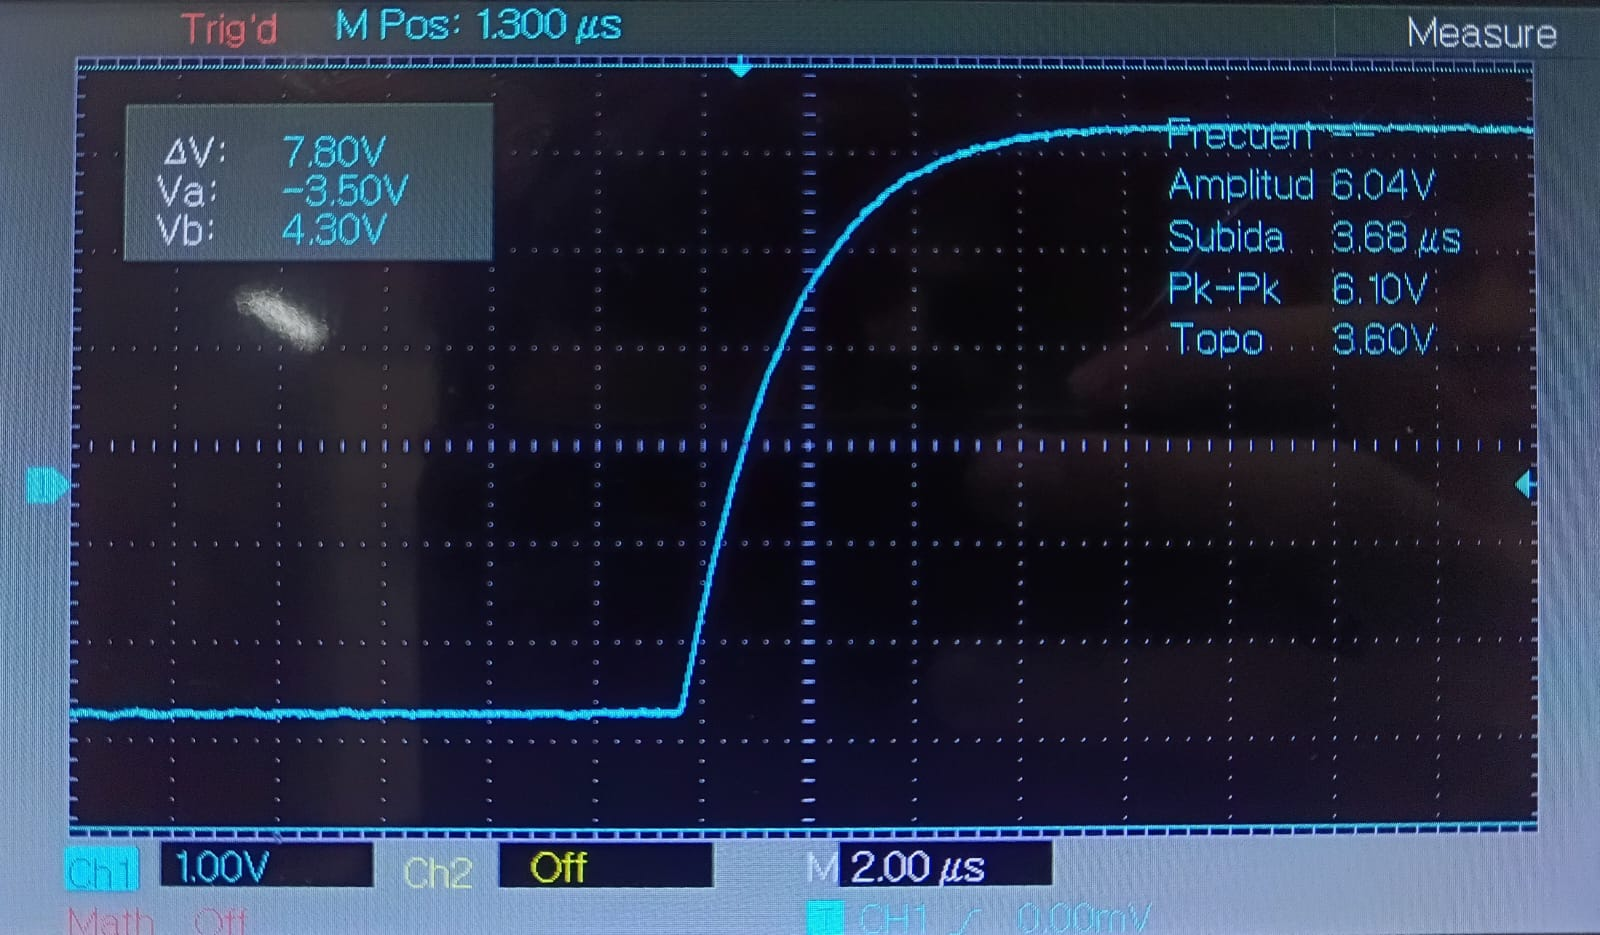
\includegraphics[width=1\textwidth]{Imagenes/tcLA.jpeg}
        \caption{Lazo Abierto}
        \label{fig:tcLA}
    \end{subfigure}
    \hfill
    \begin{subfigure}[b]{0.54\textwidth}
        \centering
            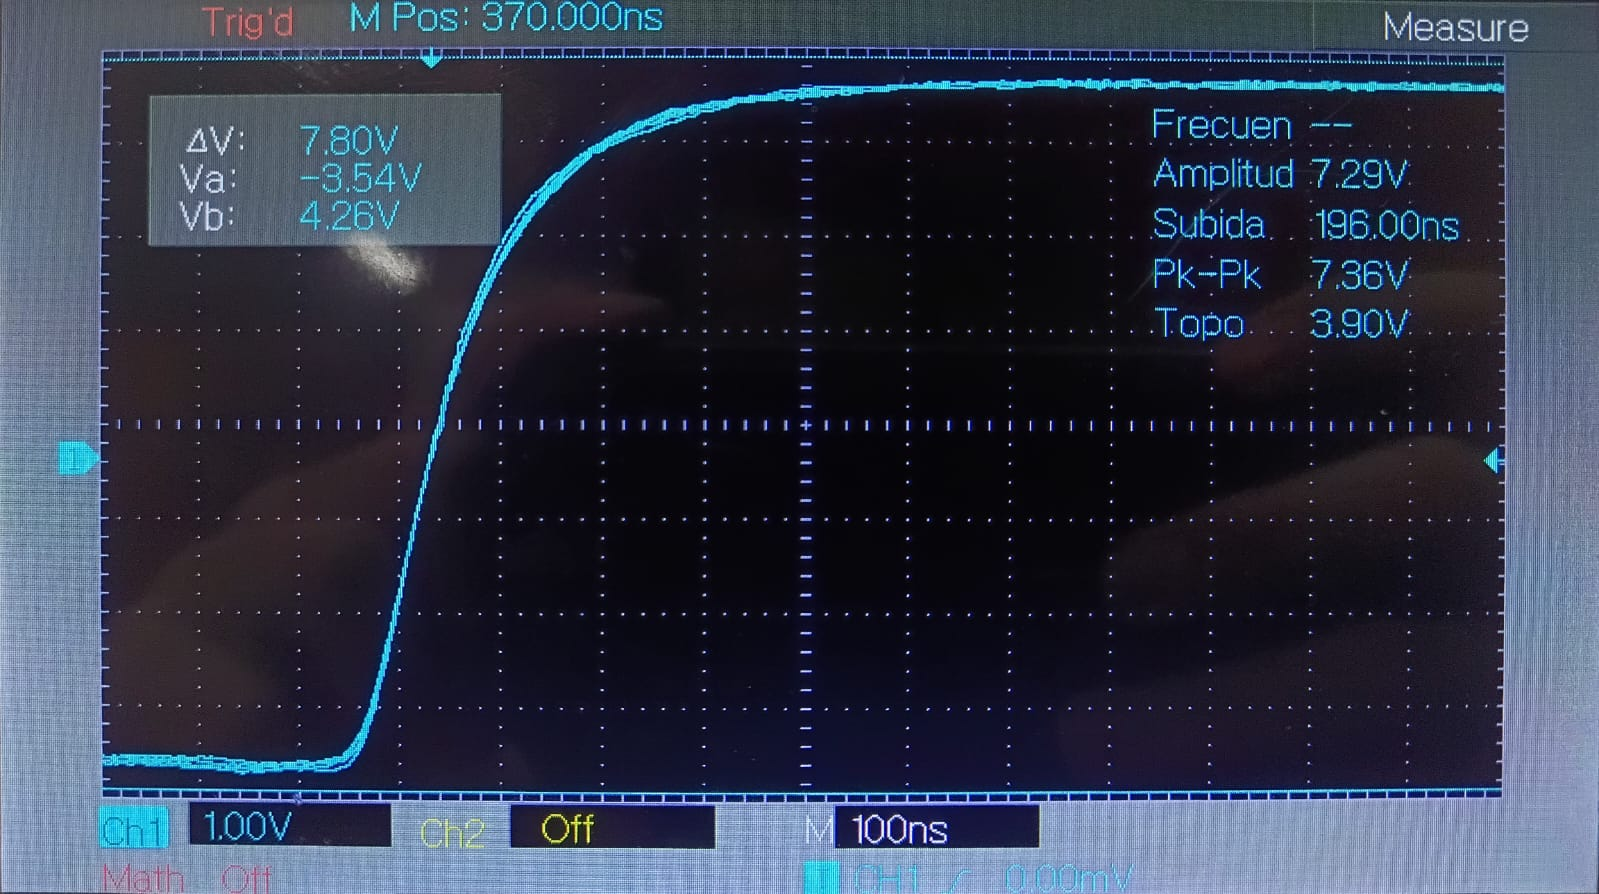
\includegraphics[width=1\textwidth]{Imagenes/tcLC.jpeg}
        \caption{Lazo Cerrado}
        \label{fig:tcLC}
    \end{subfigure}
    \caption{Flancos ascendente y tiempos de subida para cada configuración}
    \label{fig:tc}
    \end{center}
\end{figure}

Los valores obtenidos en cada caso fueron:

\begin{equation*}
    t_{c_{LA}} = 3,68 ~\mu s
    \hspace{1cm} y \hspace{1cm}
    t_{c_{LC}} = 196 ~ns
\end{equation*}

\subsubsection{Cálculos}

A partir de estos valores, se calculará el ancho de banda del amplificador. Pero antes de eso, se debe corroborar que el tiempo de subida, no sea comparable con el del osciloscopio, para lo cual se debe averiguar el tiempo de subida de este último. Para esto se utilizará la ecuación \ref{eq:tc_osc}, expuesta en el Marco Teórico. 

Para este experimento se utilizó el osciloscopio digital de la marca UNI-T, modelo UTD2102CEX. El ancho de banda de este osciloscopio es de 100 MHz.

\begin{equation*}
    t_{c_{osc}} = \cfrac{0.35}{AB_{osc}}
    \hspace{5mm} \Longrightarrow \hspace{5mm}
    t_{c_{osc}} = \cfrac{0.35}{100 \cdot 10^6 Hz} = 3.5 ns
\end{equation*}

Para el primer caso, amplificador a lazo abierto, el tiempo de crecimiento es mucho mayor que el recién calculado, por lo que no hace falta realizar la corrección. Además, del experimento anterior conocemos que este modo presenta una respuesta con caída exponencial, por lo que el \textit{k} valdrá 0,35. Partiendo de la ecuación \ref{eq:ABtc}, se tiene:

\begin{equation*}
    AB_{LA} = \frac{k}{t_{c_{LA}}} = \frac{0.35}{3.68 \cdot 10^{-6} [s]} = 95.109 kHz
\end{equation*}

Se aprecia que el ancho de banda obtenido, se aproxima al ancho de banda obtenido en el experimento anterior para este modo del amplificador.

Para el caso del amplificador realimentado, se tiene un tiempo de crecimiento bastante menor, el cual si puede llegar a verse afectado por el del osciloscopio. Por lo que aquí si se aplicará la ecuación de corrección (ecuación \ref{eq:correc}).

\begin{equation*}
     t_{c_{LC_{corr}}} = \sqrt{[t_{c_{LC}}]^2 + [t_{c_{osc}}]^2} = \sqrt{[196 \cdot 10^{-9}]^2 + [3.5 \cdot 10^{-9}]^2} = 196.03 ns
\end{equation*}

Finalmente, a partir de este valor y de los resultados del ejercicio anterior que demuestran que la respuesta tiene nuevamente una caída exponencial (k = 0,35), se calcula el ancho de banda del amplificador a lazo cerrado:

\begin{equation*}
    AB_{LC} = \frac{k}{t_{c_{LC_{corr}}}} = \frac{0.35}{196.03 \cdot 10^{-9} [s]} = 1.785 MHz
\end{equation*}

En este caso también se verifica que el cálculo se aproxima bastante a las mediciones de la experiencia anterior, por lo que se puede asumir que esta correctamente planteado.
